\section{Introduction}
% Main Ideas:

% IEAs
% Human Based Computation
% C-IEAs
% Problems
% Volunteers 
% Human Centered
% C-IEA Complex Interactions
  % User -> Human
  % Social Network
  % Devices IoT
  % Activities
  % Engagement

% Why an HC Framework (Objectives)  
% Presentation 


% IEAs
Interactive evolutionary computation (IEC) systems are, in general, evolutionary methods
whose fitness evaluations are performed by humans through an interactive system \cite{eiben2015interactive}.
They are usually applied in problems where the fitness function is not known  or simply
does not exist, and the result of optimization should fit certain human need. That is why their use 
case includes the evolution of objects with subjective characteristics such visual appeal or 
attractiveness \cite{biomorphs} as well as others where human behavior is 
considered, for instance to optimize teamwork \cite{kosorukoff2002evolutionary}
or creativity cite[cook].
% Human Based Computation
These IEC systems are an interesting venue of research, since they have demonstrated their ability for effectively 
producing art and design \cite{Bentley:1999:intro,Sims:1991,todd:1992,evoeco},
as well as other artifacts in many other domains \cite{ie1}. In these cases when 
human interaction is responsible of other 
operations of the evolutionary process some authors classify these IEC methods 
as human-based evolutionary computation cite[kosorukoff] or as human-based computation cite[].
% Problems
However, the necessary intervention of humans, brings certain challenges to designers of IEC methods  
namely, human evaluations are slow and expensive, there is a
human fatigue caused by the interaction \cite{ie1}, and
there is also the boredom arising when users evaluate a large number of phenotypes 
many of which are not interesting or are very similar to each other.
% C-IEAs
Moreover, the performance of theses systems effectively depends on the number of users
they are able to include; and in order to reach more human users,
Interactive Evolutionary Algorithms (IEAs) are 
some times developed as web applications depending on visitors to the web to interactively help
with the search, using both anonymous and registered users. Some systems 
employ a collaborative technique, where several users assign a quality assessment 
to a single solution and then an aggregated fitness value is calculated 
\cite{picbreeder,seyama2016development,wagy2014collective}.
%The number of evaluations that IEC can receive is limited by the number of users
%collaborating and the amount of interaction of each. 
Having a volunteer system  can lower the requirements of anyone participating in
the experiment thus increasing the {\em performance}, in terms of {\em
human brain cycles}, of the whole system.
% Volunteers 
Using a volunteer based system raises other issues \cite{sarmenta2001volunteer,web:BOINC}, 
such as the volunteer\'s lack of accountability,
and the need to build trust between participants and application
providers. Issues for the provider of the system or organizer  are also the difficulty of establishing 
the amount of time and resources
a volunteer is willing to spend on the system, and how they decide if they
participate or not \cite{JJ:2016}. 

% Human Centered
In order to increase volunteer participation and to tackle some of the issues mentioned above,  
we proposed a software framework following a human centered design \cite{greenhouse2012human},
giving extensive attention to volunteers, not only because their
explicit evaluation is essential, but also because the context of the 
interaction affects the system as a whole.
%Evolutionary computation algorithms are data driven since it is important to keep data about the 
%population of each generation, in order to generate the next or even change certain parameters
%or analyze the evolutionary process. 
% Human Centered Importance
%The framework models the context of interaction along with the population and
%this knowledge is available to be an integral part of the evolutionary computation.
%This could be generalized?
For example, in a C-IEC application, fitness assignment depend on the
actions of a social network of users.  Actions are triggered when 
they tag, share, rate, store or even delete a phenotype. 
The selection of parents could depend on the previous actions, leveraging information 
such as the fact that they have the same tag, or where shared by
similar users.
% IoT
%The context of interaction, can also include data retrieved from sensors and other IoT devices.
% Engagement
Data available from the interaction is also used to increase the performance of the system by applying 
gamification techniques. Gamification is defined by Deterding et al. \cite{deterding2011game} as
\begin{quote}
  the use of game design elements in non-game contexts.
\end{quote}  
The gamification element employed in this case study has been a rewarding mechanism  
\cite{dubois2013understanding}. In general rewards  consist of a reputation system with score points, 
levels and leader boards. Points are awarded to users in response of 
the accomplishment of certain activities that need to be encouraged. Levels depend
on the score and certain features of the game are only available to gamers when 
they reach a giving level. % Say what we are doing in this case - JJ

Three case studies are presented as a proof of concept, providing both
conceptual and implementation details of the framework. 

The rest of this paper is organized as follows.
Section \ref{sec:related} presents related work on the topic 
of Interactive Evolution.
Then, Section \ref{sec:framework} presents the framework of Human Interactions in Collaborative Interactive 
 Evolutionary Computation which 
the main proposal of this work. An implementation using the ES-I framework 
is detailed in Section \ref{sec:implementation}.
The case studies  and results are presented in Section \ref{sec:experiments}.
Finally, a concluding remarks are provided in Section \ref{sec:conclusions}.

\section{Related Work}
\label{sec:related}

An early example of web based collaboration is the work by 
Langdon \cite{langdon:2004}, which evolved fractal representations of virtual creatures. 
Similarly, Secretan et al. \cite{picbreeder} and Clune and Lipson \cite{forms} use web-based IEAs 
to evolve artistic artifacts using a generative encoding, compositional pattern producing networks.
Another example was the Galapagos Project \cite{sims1997interactivity},
an exhibit in the Tokyo Multimedia Museum (1997--2000) were visitors interacted with images presented in 
twelve displays by selecting those they found most aesthetically interesting by standing on
step sensors in front of them. 
% C-IEAS
Given the fatigue fitness evaluations produce in human users when applying IEAs, some authors have tried to mitigate
the problem by allowing the algorithm to collaborate with the user, so that sometimes users perform the evaluation, 
but also specific measures are included into the algorithm to perform the evaluation of some features automatically.  
For instance, Reis et al. added some terrain measures (such as accessibility and edge length) to a standard 
IEC in \cite{DBLP:journals/soco/FradeVC12} .  This way the algorithm was capable of providing terrains that would
otherwise have need users evaluation for these specific features. Seyama and Munetomo \cite{seyama2016development}
also propose the reduction of the user fatigue by using a collaborative filtering algorithm to show only the
information utilized by similar users as they collaborate with a large number of users for 
the interactive modeling of 3D glasses. 

Some Collaborative IEC (C-IEC) systems promote user engagement by presenting interesting information to 
users, for instance the genetic lineage of each phenotype or the most popular or 
best rated solucion\cite{picbreeder,forms}.In a recent work by 
Wagy \& Bongard \cite{wagy2014collective} user interaction is needed for evaluating the fitness and developing
new designs of robot locomotion. Collaboration is encouraged by gamifying the system 
using the maximum distance indicator to inspire the user to try and ``beat'' previous designs. 
In any case, using gamification techniques imply that we must deal with interactive evolutionary
system as socio-technical constructs, where the social aspects are
essential to understand its dynamics. In this sense, conclusions
reached with other systems such as NodEO \cite{DBLP:conf/gecco/MereloCGCRV16} can also be applied to this
system; and applying social network techniques such as graph analysis
to their study will allow us to understand them more thoroughly. 

Collaborative IEC (C-IEC) systems also need to store highly connected data, as it is common in current applications
like social networks. In order to deal with large datasets of connected data found in these systems,
graph databases \cite{angles2012comparison} have been proposed as an alternative to relational databases 
which have performance limitations when dealing with highly connected data \cite{holzschuher2013performance}.
The framework and data model for representing the interactive process of C-IEC systems is proposed next
% Volunteer Based
% HBC
% Engagement Techniques
% Models

\begin{figure*}[!t]
    \centering
        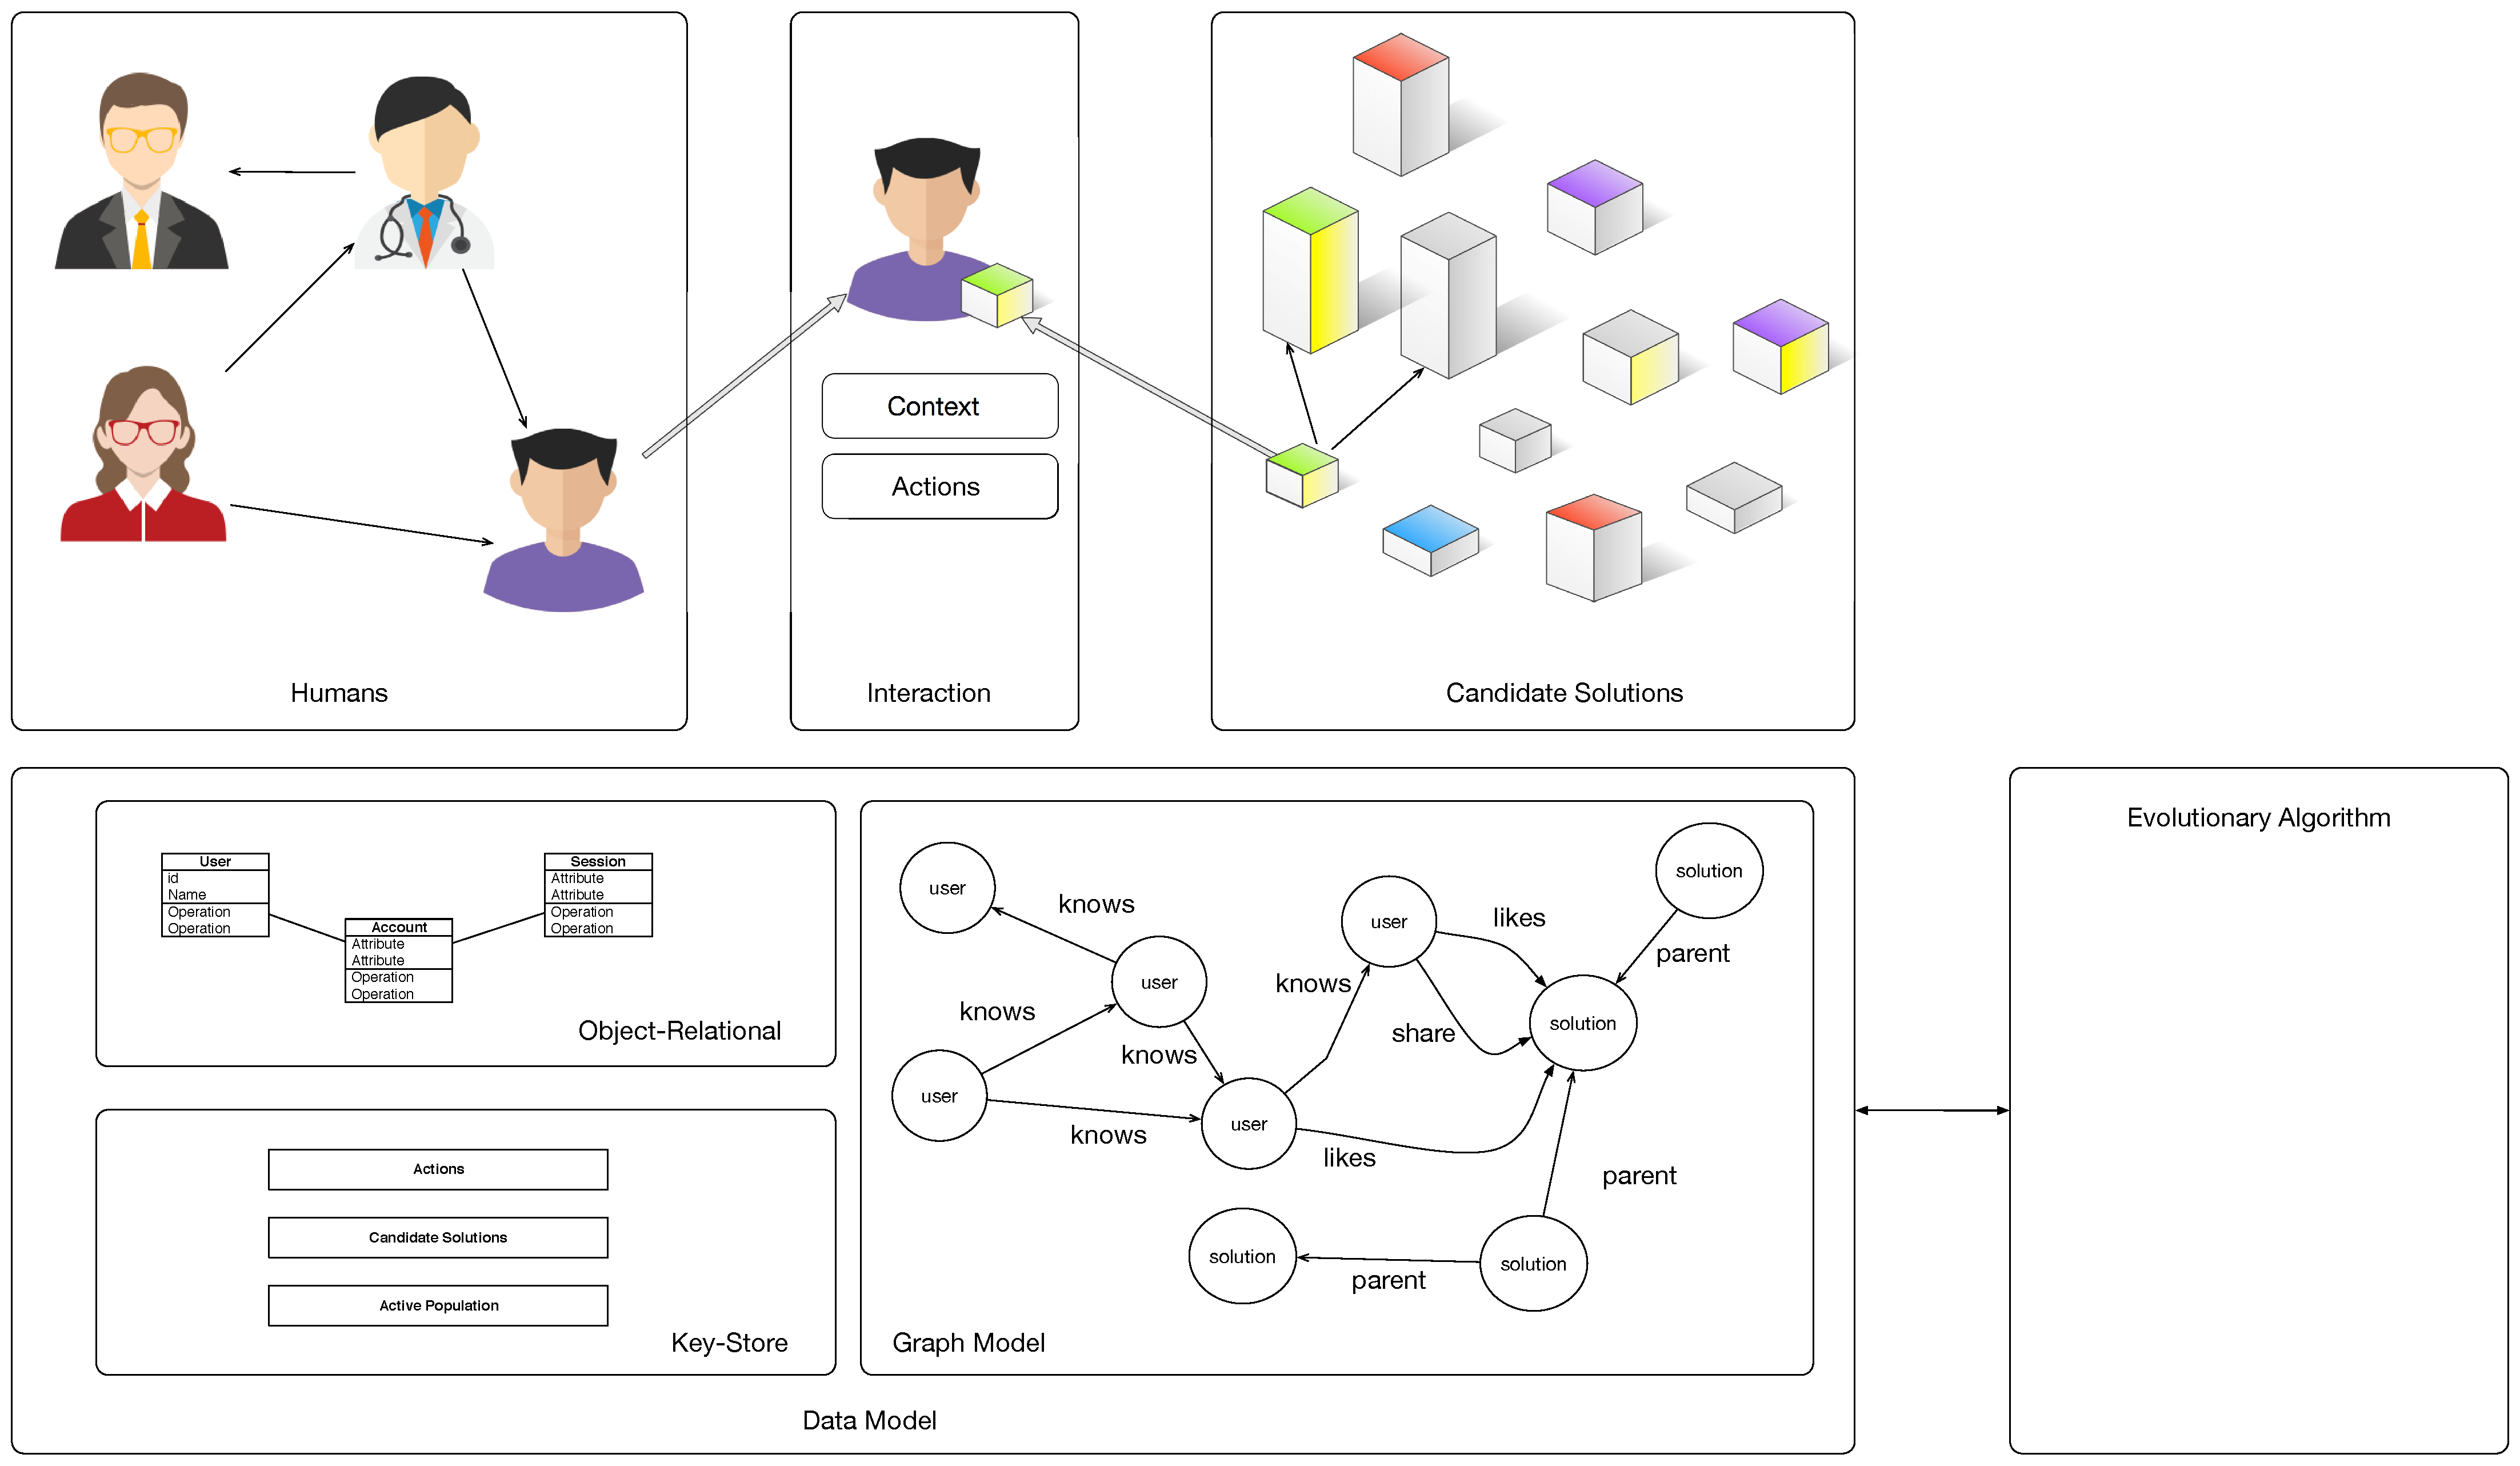
\includegraphics[width=5in]{img/framework.eps}
    \caption{IEC Human-centered framework.}
    \label{fig:hc_framework}
\end{figure*}

\section{Human-Centered IEC Framework}
\label{sec:framework}
% Comment: 
% Maybe in this case we should use the term software framework or architecture. 
The general goal of this line of research is to develop a human-centered \cite{gasson2003human} 
software framework for interactive evolutionary computation (IEC). 
A framework is defined as a reusable architectural design together
with an implementation \cite{campbell1991choices}, in this case 
providing generalized components to developers of IEC systems. 
% Just by saying is Human Centered this is not needed, it was from the User-Centered days - Mario
%In the
%description below %below? If that's te chase, we _will_ - JJ
% Not only in the description, more like a paradigm shitf. But ok for now - Mario
% we will deliberately use the more general 
%term Human instead of User, because humans are not always playing the role of users in software engineering sense, they
%could just be interacting naturally with their environment and
%unwittingly and at the same time they are implicitly
%evaluating a possible solution.  

%Which framework? Are we talking about a particular framework or that
%is the general rule for frameworks? - JJ
%Is general bu I was talking about this one - Mario
The proposed framework includes components that can be refined to increase
participation and also to minimize the amount of evaluations needed for the evolutionary 
process in a given IEC application. Software frameworks often have a vison or a way 
of thinking \cite{carneiro2010introducing} guiding their
design. Before diving into details the main design considerations of the
framework are explained next:  % constraints? Rules? You don't decide
                               % that users are humans, they simply
                               % are - JJ 
                               % Ok, is more like we want to acknowledge that, 
                               % considerations? - Mario


\begin{itemize}
\item {\bf Users are human} 
  The framework follows the approach of human centered computing \cite{sebe2010human},
  in which the context, environment, interfaces, preferences, accessibility, human relations, cognitive
  limitations, culture, creativity and other human aspects are an integral part of the system.
  Humans are the computing resorces of the system, having unique characteristics as those identified by 
  Sun \& Dance \cite{Sun2013}
\begin{quote}
  (1) humans can solve computer hard problems; (2) humans are very good at exception handling, (3) humans have creativity, (4) humans have cognitive load limitation, (5) humans are vulnerable to 
  psychological manipulation, (6) humans are prone to errors,
  especially for reflective tasks.
\end{quote}  


\item {\bf Users are volunteers} Users donate their computing resources, so they are unaccountable, 
  some times they try to game the system. Project owners must actively promote and design the interactive
  system to engage volunteers \cite{oh2015clicking}. % Define
                                % providers somewhere. Experiment
                                % owners? - JJ
                                % Using project, like BOINC  https://boinc.berkeley.edu/trac/wiki/VolunteerComputing - M

\item {\bf Users are not alone}
  Relationship between users in an interactive evolutionary algorithm can be modeled
  as a social network, with well established semantics, algorithms and metrics \cite{ahuja1993network}.
  A graph model could enable researchers to find other ways of identifying leaders of 
  opinion or measuring the similarity between user's preferences. 
  These measures can then be used by recommender algorithms selecting 
  phenotypes according users' preferences. 

\item {\bf Context of use matters}
  \textit{Context} In computer science Fischer \cite{fischer2012context}
  defines context as
  \begin{quote}
  the interaction between humans and
  computers in socio-technical systems that takes place in a certain
  context referring to the physical and social situation in which
  computational devices and environments are embedded.
\end{quote}   
  Fischer also identifies the important aspects to consider when the context is used: how it is
  the contextual data obtained, how the context is represented and what
  goals and purposes the context has when is used in a particular
  application.   An IEC system will  be used within a certain range of technical, physical and social or
  organizational environments \cite{maguire2001context} that may affect its use.
  The concept has been formally defined
  by ISO standard 9241-11 \cite{international1998iso} as\begin{quote}
  users,
  tasks and equipment (hardware, software and materials), and the
  physical and social environments in which a product is used.
\end{quote}

\item {\bf Interaction is a stream of actions}
  Real time processing of users' actions could be needed for certain applications when data is 
  captured by sensors, or directly captured as user input. For example, social networks keep track of 
  users' interactions with other users, media objects and places. Users of 
  social networks (for instance the Facebook Graph) are accustomed to express these 
  complex relationships in sentences such as: ``John and Ann eating breakfast at Tony's''. 
  Other example is the W3C Activity Streams 2.0 specification used for representing activities 
  common in social web applications \cite{json:streams}. 
\end{itemize}

% Say something about how this is important for the framework and how
% you incorporate it - JJ
% Done - Mario
The above considerations have guided the design of the framework, and througout they have been
treated as application constraints. In order to satisfy theses requirements the
human centered IEC architecture consists of three high level components depicted
in figure \ref{fig:hc_framework}:

\begin{itemize}
  \item {\bf Interactive Evolutionary Computational system} 
  This is the real world system that we are going to represent in the data model, 
  it consist of human users and their interactions with one or more phenotypes
  from the population. There are many ways in which humans could interact 
  with phenotypes. The interaction consists of a set of actions and 
  takes place in a certain context. For example, through a mobile device  
  or by interacting with real world objects 
  \cite{de2014artists,de2013unplugging}. 
  There is also the possibility that fitness or even part of the search 
  is done by devices lent by humans \cite{DBLP:conf/gecco/MereloCGCRV16}.
  The information gathered through the interaction is the primary concern
  as it will guide the search. 

  \item {\bf IEC Data Model}
  A data model is used to describe the IEC system prior to a physical 
  implementation.  Depending on the domain several techniques can be used.
  Parts of the system could be better described by an Entity relationship 
  modeling to be used in a relational database or a class digram for a 
  key-value store. A graph is proposed for modeling the social network of users 
  and their interaction with the population. When implemented a graph database 
  will be the back-end of the system. 

  \item {\bf Evolutionary Algorithm} 
  The EA algorithm interacts with the data model. The EA could also be done with the help of
  humans, for instance in the XY project \cite{de2013unplugging} artists actually painted
  the solutions of the new population.  
\end{itemize}

\section{Data Model Implementation}
\label{sec:implementation}

The core of the framework is the data model because both the IEC system and the EA will 
depend on the application. In this section implementation details of the Data Model are presented.
Three database models are employed to store different elements of the system: 

  \subsection{EvoSpace-Redis}
EvoSpace is a population store \cite{Evospace}  for the development of 
evolutionary algorithms that are intended to run on a cloud computing model. 
The population is decoupled from any particular evolutionary algorithm. 
Candidate solutions are stored as of objects in a population, and they can be withdrawn, 
processed and replaced using a specified set of methods \cite{GValdez2015}. The population
is stored in-memory, using the Redis key-value database. Redis was chosen over a relational 
database management system, because it provides a hash based implementation of sets and 
queues which are natural data structures for the EvoSpace model. Basicaly a sample of 
candidate solutions are retieved from the server, evaluated, and then sent back. 
The same operations are used to Evolve the population. In EvoSpace individuals replaced 
in the population are stored indefinitly, to permit users to store permalinks to them.
Implementation details are presented in \cite{garcia2013evospace}.

\subsection{Graph-Neo4J}
  In order to deal with large datasets of connected data found in these systems,
  graph databases \cite{angles2012comparison} have been proposed as an alternative to relational databases 
  which have performance limitations when dealing with highly connected data \cite{holzschuher2013performance}.
  A graph is proposed for modeling the social network of users, their interaction with 
  candidate solutions, and the relationships between them in the population.
  The graph database system used in the implementation is Neo4J as it is
  a scalable solution \cite{miller2013graph,holzschuher2013performance}, and well supported and documented
  in PaaS infrastructures like Heroku. The Cypher query language it used to retrieve views from the graph.
  An exaplmple query is shown in figure \ref{fig:cypher} where the relations between users and solutions 
  are presented.
  
  \begin{figure}[!t]
    \centering
        \includegraphics[width=3.5in]{img/gui-neo.png}
    \caption{Example query in Cypher.}
    \label{fig:cypher}
  \end{figure}

\subsection{Relational Objects-PostgreSQL}
  The PostgreSQL relational database system is also employed because user sessions and authentication,
  as well as dynamic web pages are handled directly by the Django web
  framework \cite{garcia2013evospace}. % these implementations details
                                % could go if needed. 

\subsection{Interfaces}
The appropiate human interface will depend on the application domain, the current framework implemantation  
employs a web based application. Developers can use different templates, to present one or more phenotypes 
at a time, and the type of rating system: like or one to five stars. Another implementations do not need a
graphical interface at all, for example the EvoDraw instalation or the XYZ Project \cite{de2014artists}.   
    
\subsection{Evolution}
The evolutionary algorithm is decoupled from the data model, the algorithm can be implemented as an
EvoWorker \cite{garcia2013evospace}, use an external library, or even it can be done by humans.
An additional tool was implmented for a human based evolution , where volunteers select the parents of
the next generation and upload the new individuals \cite{de2014artists}.  

\section{Case Study: EvoDraw}
As a case study, a IEA was developed using the 
EvoSpace-Interactive (ES-I) platform \cite{garcia2013evospace}
A brief description of the application is presented next, focusing
on the data elements that where ported to the graph model.

\begin{figure}[!t]
    \centering
        \includegraphics[width=3.5in]{img/interface.png}
    \caption{User interface of the EvoDrawings application.}
    \label{fig:web}
\end{figure}

\label{sec:experiments}
\begin{figure}[!t]
    \centering
        \includegraphics[width=3.5in]{img/interfaceXYZ.png}
    \caption{User interface of the XYZ application.}
    \label{fig:xyz}
\end{figure}

\subsubsection{Fitness Assignment}
\label{sec:assignment}
% changed to this, because I understand it does not always work that
% way - JJ
The ES-I platform has been programmed to employ a collaborative methodology for performing fitness
 assignment. Several registered users assign a quality assessment to a single
phenotype and then an aggregated fitness value is calculated,
depending on the rating (from 1 to 5 stars) by each particular user,  % how do you define
                                % "taste"? - JJ
                                % Using actions
resulting in a many-to-many relationship between users and
phenotypes. 
 %scored by them? - JJ 
Other components or users of the systems can 
query this user-phenotype relation to extract relevant
knowledge about the process and the population, for instance showing the
most popular phenotype, or the the user with more participation 
\cite{picbreeder}.
In order to do this, metadata about phenotypes 
must be permanently stored, even
if they are no longer in the active population. 

\subsubsection{Collaboration}
\label{sec:col}
Users need to authenticate themselves to the system using their
Facebook account. In that sense, some users might not be interested
either because they do not want to give that information or simply because
they do not use that particular social network. Even as we might lose
some users that way, the additional information we obtain for scoring
phenotypes more than compensates for that. 
After entering the web application by using their Facebook account,
users can collaborate with their Facebook friends, 
sharing those phenotypes they like, or by taking phenotypes
from their friend's collections by using the web interface depicted 
in Figure \ref{fig:web}.
At the top left corner a list of Facebook friends is presented
to encourage users to interact with the system. In the central 
\emph{ Wall } area, a phenotype sampled from the population that is
being evolved via the evolutionary algorithm 
is shown to the user.
Here, the user can interact with the system in two ways.
First, he can assign a rating to the phenotype using
a five star rating system or,
additionally, a user can choose to add an image to one of their \emph{Collections}.
A collection is a special folder that stores those phenotypes a user likes and wishes
to save. After the user finishes interacting with the phenotype
on the Wall, he can choose to retrieve a new one from the population.
At the left hand side of \ref{fig:web}, the web page shows the \emph{Collections} section.
The user can create several collections, to group and organize his favorite 
artifacts. Moreover, users can browse the content of each collection and from
there share images through their social network.
When a user hovers the cursor over a phenotypes a pop-up pane shows how many users have
liked the phenotype. The pane also includes a link to the phenotype's 
details, the parents, genetic operators that created it, and genealogy
information. This makes the assignment of fitness through the rating
system a {\em social} activity, pursuing the objective of this work,
which is to increase engagement of the users.


\subsection{Graph Model} 

The graph model for the EvoDraw applications has the following types of
nodes: {\bf User}, {\bf Phenotype} and {\bf Collection} . The Collection node represents
a collection of drawings belonging to users. One collection can contain many phenotypes 
or be empty and a single phenotype could be shared by many collections. The interaction 
between these entities are represented by the following edges:

\begin{itemize}
\item {\bf Likes} This relation describes the interaction between a user and
a phenotype in which a rating value is assigned this is represented by 
the {\tt rate} attribute. In the current application a user is allowed to rate
a phenotype multiple times, so the date of the interactions is also of
interest.

\item {\bf Knows} The relation connects two users that know each
other in the Facebook social graph. 

\item {\bf Parent} Describes what phenotype is the parent of a new
  phenotype. 

\item {\bf Has} The relation describes an ownership relation between users and
those collections they own. Also a collection {\tt has}  phenotypes stored
in them.
\end{itemize}

\subsection{Gamification}
The rewarding mechanism as it is applied in EvoDraw 
consists in giving more importance to the preference of those users having a higher reputation
as given by the score points and experience levels.  

The score achieved by users depends on the actions he does in the system as
each time a user does one of these actions their score is incremented by one:
\begin{itemize}
\item Start a session.
\item Rate a phenotype.
\item Create a collection.
\item Save a phenotype of the wall to a collection.
\item Save a phenotypes from a friend's collection.
\item Explore collections of other friends.
\end{itemize}

Only the ``Start a session'' and ``Explore collections of other friends'' actions 
are not reflected in the graph model since they are stored instead in the PostgreSQL relational
database system. This is because user sessions and authentication, as well as basic
web requests, are handled directly by the Django web framework \cite{garcia2013evospace}.  

Two scores are used to determine the weight of a user's preference:
\begin{itemize}
\item {\em Experience}: This value depends on the score and is a value 
between 0 and 100. It is assumed for this case, that once a user
reaches a 100 actions, it has enough experience on using the application.   

\item {\em Participation}: This value is simply the degree of the user node 
in the graph. This measure considers the number of users he knows,
collections and phenotypes rated.    
\end{itemize}

\section{Experimental Setup}
\label{sec:experiments}
We present in this section the results of a comparison between three versions
of the same IEC application. The goal of the experiment is to compare two 
gamification techniques to increase volunteer participation against a third 
without any technique applied. The main difference between both versions employing 
gamification is how the fitness of phenotypes
is calculated and the information presented to users. 

Three versions were compared:
\begin{itemize}
\item Base (B). All users have the same weight.
\item Non Graph Gamification (G). Only experience is considered
\item Graph Gamification (GG) . Both experience and participation are considered.
\end{itemize}
When gamification was employed, all score values known where presented to users
and a ranking of users by weight was shown in a window.

The three versions of the EvoDrawing web application were deployed to the
Heroku cloud service with the same configuration: using the
Heroku Free option with a 512 MB of RAM, adding only the GrapheneDB and RedisTOGO plug-ins.
Table \ref{tab:params} shows the parameters used for the evolutionary algorithm. The graph database 
system used in the implementation was Neo4J as it was already available as a plug-in in Heroku, is well documented
and a scalable solution \cite{miller2013graph,holzschuher2013performance}.  

\begin{table}
  \small
  \caption{ Parameters for experiments.  }
  \label{tab:params} 
  \centering
  \small
  \begin{tabular}{l  c   }
    \hline\noalign{\smallskip}
     Parameter & Value \\
    \noalign{\smallskip}\hline\noalign{\smallskip}
    Initial Population Size   & 80 \\ \hline
    Sample Size & 1 \\ \hline
    Step Size & 8 Samples \\ \hline
    Mutation &  \\ \hline
    Selection & Tournament \\ \hline
    Tournament Size &  6 \\ \hline
  \end{tabular}
\end{table}

% Anuncements
At the start of every experiment, a call to participation was issued
through social networks, 
particularly on Facebook and Twitter.
It is important to note that volunteers needed to log-in to Facebook and give permissions to the 
web application in order to participate, in this case there were no anonymous volunteers. This enabled the automatic access to
each participant's social network and enabled the system to store a local copy of those friends participating.
However, another experiment would be needed to see the effect this
requirement has on participation, since we are not dealing with it in
this paper. 

The link used in the call for participation
was shortened Google URL, that provides metadata and analytics for the
users that click on it. 
In table \ref{tab:urls} the URL for each deployment in the Heroku platform is shown,
along with the short URL and the analytics link. In the same table a link to the GitHub 
application repository used to deploy to Heroku is also listed.    
%Isn't this anonymous? - JJ
% like in double blind? I think so, that is why no link is given in the table. - Mario 

\begin{table}
  \small
  \caption{ Deployment data. URLs were {\tt
      evodrawings0(1,2,3).herokuapp.com}. For analytics URLs, add {\tt
    .info}.}
  \label{tab:urls} 
  \centering
  \small
  \begin{tabular}{l l l }
    \hline\noalign{\smallskip}
     Deployment &  Shortened URL &  Github Repository \\
    \noalign{\smallskip}\hline\noalign{\smallskip}
    B   & goo.gl/jLis4Q &   \\ \hline
    G   & goo.gl/jqjNy5 &  \\ \hline
    GG  & goo.gl/J8TCe1 &   \\ \hline
    \end{tabular}
\end{table}

Only data for the first week of deployment was considered for the experiments, and they where conducted 
between January and May of 2016. 

\subsubsection{Results} 
Before launch, each deployment was first tried with a few beta testers. When applying the leader board
gamification technique for the first time a problem was found in this stage. The problem was that some 
users were cheating by giving a rating to an animation even before it was returned from the server, this was done by just
constantly clicking the mouse button. This is a common problem found in systems using leader boards because
by making the scores visible to other players they are encouraged to compete \cite{hickman2010total}. 
According to \cite{kumar2013gamification} best-practice gamification designs try to
refrain from using this element because of  problematic consequences of competition, which can result 
in negative conduct, low cooperation and collaboration, or disadvantaging certain player
demographics such as women. In order to still measure the effect of the leader board on the system, the 
problem of cheating was mitigated by disabling the rate button for a certain amount of time giving the animation
enough time to finish. But the problem persists, competitive users will try to get in to the leader board by other means.

The results of each of the three experiments in terms of participation are detailed next.

\subsection{ Base deployment}
After a week of the announcement the total number of volunteers for this experiment was 53 registered users. 
The total number of nodes generated in the graph was 595, with a total of 2220 relationships. In this
experiment a total of 500 new phenotypes where generated. The total number of evaluated
phenotypes for each volunteer is presented in figure
\ref{fig:top-ranked-participation} in blue. Users are ranked by
the number of phenotypes they rated, in the \emph{x} axis is the rank, and in the \emph{y} axis 
the number of phenotypes evaluated using a logarithmic scale.   % Ranked by... - JJ
% Done - Mario


\subsection{ Non Graph Gamification deployment}
The total number of volunteers for this experiment was very close to
the one obtained in the previous
experiment: 54 registered users. The total number of nodes generated in the graph was 648, 
with a total of 2596 relationships. These numbers are close to those obtained in the base experiment,
with a marginal increase in participation. The increased participation also helped in the creation of
more phenotypes for a total of 648. The total number of evaluated
phenotypes for each volunteer is presented in figure \ref{fig:top-ranked-participation} in red. 

\subsection{ Graph Gamification deployment}
This experiment had the higher number of volunteers for for a total of 68 registered users. 
In this experiment a total of 3594 new phenotypes where generated in the experiment. 
The total number of evaluated phenotypes for each volunteer is presented in figure 
\ref{fig:top-ranked-participation} in green. 

The results presented in figure \ref{fig:top-ranked-participation}, show that those users with
higher level of participation in deployments B and G, had about the same behavior, but the difference
came with users with medium level of participation, in this case participants where more engaged in deployment
G. When comparing all the experiments the deployment GG had the higher number of participation in users
of all levels.    

\section{Results}
Before launch, each deployment was first tried with a few beta testers. When applying the leader board
gamification technique for the first time a problem was found in this stage. The problem was that some 
users were cheating by giving a rating to an animation even before it was returned from the server, this was done by just
constantly clicking the mouse button. This is a common problem found in systems using leader boards because
by making the scores visible to other players they are encouraged to compete \cite{hickman2010total}. 
According to \cite{kumar2013gamification} best-practice gamification designs try to
refrain from using this element because of  problematic consequences of competition, which can result 
in negative conduct, low cooperation and collaboration, or disadvantaging certain player
demographics such as women. In order to still measure the effect of the leader board on the system, the 
problem of cheating was mitigated by disabling the rate button for a certain amount of time giving the animation
enough time to finish. But the problem persists, competitive users will try to get in to the leader board by other means.

The results of each of the three experiments in terms of participation are detailed next.

\subsubsection{ Base deployment}
After a week of the announcement the total number of volunteers for this experiment was 53 registered users. 
The total number of nodes generated in the graph was 595, with a total of 2220 relationships. In this
experiment a total of 500 new phenotypes where generated. The total number of evaluated
phenotypes for each volunteer is presented in figure
\ref{fig:top-ranked-participation} in blue. Users are ranked by
the number of phenotypes they rated, in the \emph{x} axis is the rank, and in the \emph{y} axis 
the number of phenotypes evaluated using a logarithmic scale.   % Ranked by... - JJ
% Done - Mario


\subsubsection{ Non Graph Gamification deployment}
The total number of volunteers for this experiment was very close to
the one obtained in the previous
experiment: 54 registered users. The total number of nodes generated in the graph was 648, 
with a total of 2596 relationships. These numbers are close to those obtained in the base experiment,
with a marginal increase in participation. The increased participation also helped in the creation of
more phenotypes for a total of 648. The total number of evaluated
phenotypes for each volunteer is presented in figure \ref{fig:top-ranked-participation} in red. 

\subsubsection{ Graph Gamification deployment}
This experiment had the higher number of volunteers for for a total of 68 registered users. 
In this experiment a total of 3594 new phenotypes where generated in the experiment. 
The total number of evaluated phenotypes for each volunteer is presented in figure 
\ref{fig:top-ranked-participation} in green. 

The results presented in figure \ref{fig:top-ranked-participation}, show that those users with
higher level of participation in deployments B and G, had about the same behavior, but the difference
came with users with medium level of participation, in this case participants where more engaged in deployment
G. When comparing all the experiments the deployment GG had the higher number of participation in users
of all levels.


\begin{figure}[!t]
    \centering
        \includegraphics[width=3.5in]{img/weibull_1.png}
    \caption{Experiment 1. Weibull Fit}
    \label{fig:w1}
\end{figure}
\begin{figure}[!t]
    \centering
        \includegraphics[width=3.5in]{img/weibull_2.png}
    \caption{Experiment 2. Weibull Fit}
    \label{fig:w2}
\end{figure}
\begin{figure}[!t]
    \centering
        \includegraphics[width=3.5in]{img/weibull_3.png}
    \caption{Experiment 3. Weibull Fit}
    \label{fig:w3}
\end{figure}


%\subsection{EvoDraw-Kinect}
%\subsection{XYZ-Unplugged}


\section{Conclusions}
\label{sec:conclusions}

Collaborative and volunteer based IEC systems involve the dynamic 
interaction of many entities and artifacts. Employing a multi-model approach
can benefit researchers to understand and visualize this kind of systems better.
In this paper a graph model was proposed as a complement to current
models, initially to improve the visualization of different
experiments, but in this paper we prove that this model  enables
the implementation of a gamification technique to improve engagement in
a case study. Providing a common arena where users are aware of the
activities of other users in the social vicinity, as well as using
this graph to assign fitness allows in one hand for a greater
engagement by the users and from the algorithmic point of view a more
complex way of assigning fitness and push the generation of content
forward. 

One of the interesting future lines of work would be to look a bit
more closely at the behavior of users rating the system. These initial
experiments hint at a possible power law, which might indicate that
the IEC system could be self-organizing, a process that would allow it
to reach a critical state, as has been found in software repositories,
for instance \cite{Merelo2016:repomining}. The dynamics of this kind
of system are fundamentally different, and our future research will
include exploring these aspects of the system. Another line of work would be to study the negative effects of using 
gamification techniques to improve engagement, like cheating or competition.
Finally, the refinement of the proposed Human-Centered framework will need
more case studies and further multi-disciplinary research.

\begin{acks}
  % The authors would like to thank Dr. Yuhua Li for providing the
  % matlab code of  the \textit{BEPS} method. 

  % The authors would also like to thank the anonymous referees for
  % their valuable comments and helpful suggestions. The work is
  % supported by the \grantsponsor{GS501100001809}{National Natural
  %   Science Foundation of
  %   China}{http://dx.doi.org/10.13039/501100001809} under Grant
  % No.:~\grantnum{GS501100001809}{61273304}
  % and~\grantnum[http://www.nnsf.cn/youngscientsts]{GS501100001809}{Young
  % Scientsts' Support Program}.
  Reserved\\
  Space\\
  for\\
  Acks

\end{acks}
